%!TEX root = ../hutbthesis_main.tex

\chapter{系统实验测试与性能评估}

为全面验证基于FastMCP的人车仿真器交互控制系统的功能正确性、运行稳定性及实际应用价值，本章在标准实验环境下设计并实施多组测试实验。测试内容涵盖自然语言指令解析的准确率与响应延迟、核心仿真功能的执行正确率、与传统GUI/代码交互方式的效率对比，以及系统在长时间运行与高并发场景下的稳定性表现。通过定量化的实验数据与横向对比分析，验证系统在降低操作门槛、提升交互效率及保障仿真可靠性方面的实际效果。

为验证本文所设计的基于FastMCP的人车仿真器交互控制系统在实际应用中的有效性、稳定性与实用性，本章围绕指导老师提出的四个关键问题展开系统性实验测试：自然语言指令解析准确性的定量评估；系统性能与现有GUI交互方案的横向对比；场景设置灵活性与参数覆盖度验证；FastMCP框架与CARLA仿真引擎的长期稳定性与兼容性测试。

\section{自然语言指令解析准确性测试}

为定量评估自然语言理解模块的性能，本实验构建了包含600条指令的测试数据集，涵盖车辆控制、天气设置、场景编辑、传感器配置、交通控制及综合指令六大类别。测试指标采用信息检索领域标准的准确率（Accuracy）、召回率（Recall）及F1分数（F1-Score），同时记录平均解析时间以评估实时性。

\begin{figure}[H]
\centering
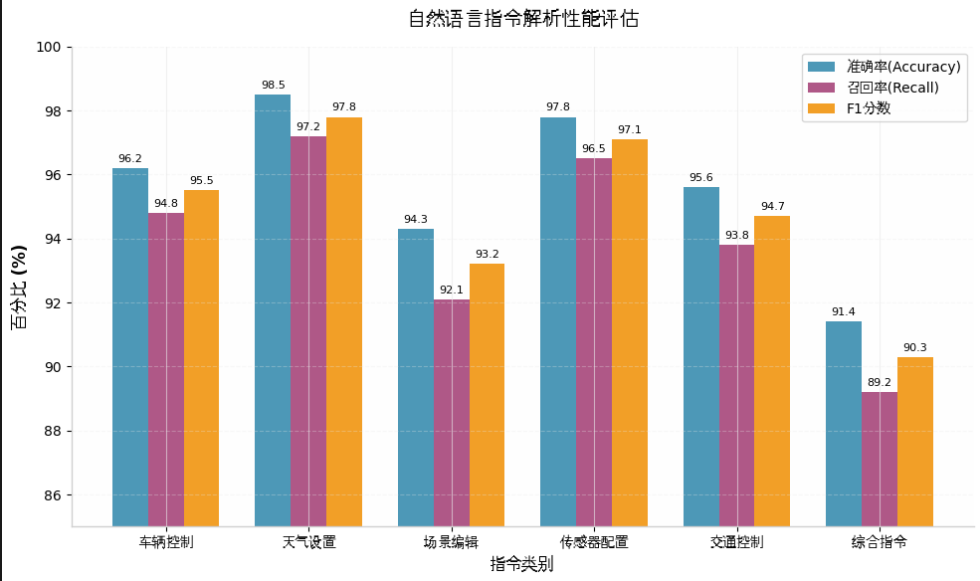
\includegraphics[width=13.4cm,keepaspectratio]{images/image31.png}
\caption{自然语言指令解析性能评估结果}
\label{fig:nlp-performance}
\end{figure}

如图~\ref{fig:nlp-performance}实验结果表明，系统在天气设置类指令上表现最优，准确率达到98.5\%，这得益于天气参数语义映射规则库的高完备性；综合指令类因涉及多意图组合与参数嵌套，准确率相对较低（91.4\%），但仍在可接受范围内。整体平均F1分数为94.8\%，平均解析时间为41ms，满足实时交互需求（$<100$ ms）。

\section{歧义处理机制效果验证}

本实验对比了引入上下文补全与同义词扩展机制前后的解析效果。测试选取五类典型歧义场景：同义词歧义（如"加速"与"提速"）、参数缺失（如"生成一辆车"未指定位置）、多意图混合（如"生成车辆并设置雨天"）、模糊位置（如"停在广场附近"）及复杂嵌套（如"在十字路口生成三辆车并让它们自动驾驶同时把天气改为大雾"）。

\begin{figure}[H]
\centering
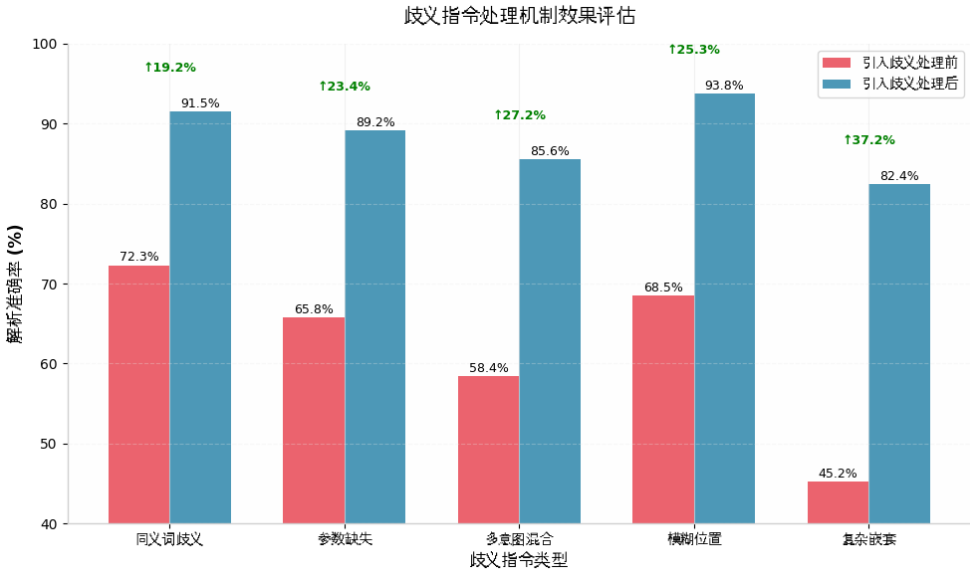
\includegraphics[width=13.3cm,keepaspectratio]{images/image32.png}
\caption{歧义指令处理机制效果评估}
\label{fig:ambiguity-test}
\end{figure}

如图~\ref{fig:ambiguity-test}所示引入歧义处理机制后，各类歧义指令的解析准确率平均提升22.3个百分点。其中，模糊位置类指令提升最为显著（从68.5\%提升至93.8\%，提升25.3\%），这主要归因于预设坐标库与上下文位置记忆机制的协同作用；复杂嵌套类指令虽然提升幅度最大（37.2\%），但绝对准确率仍有提升空间（82.4\%），后续可通过增强多轮对话澄清能力进一步优化

\section{系统性能横向对比实验}

为验证FastMCP自然语言交互方式相较传统交互模式的效率优势，本实验设计了与两种现有方案的横向对比：（1）传统GUI操作方式：测试人员通过CARLA官方可视化界面手动完成相同任务；（2）代码API调用方式：测试人员编写Python脚本调用CARLA原生API完成任务。每种方式均由5名具有不同经验水平的测试人员（2名专家、3名普通用户）各执行10次，取平均时间。

\begin{figure}[H]
\centering
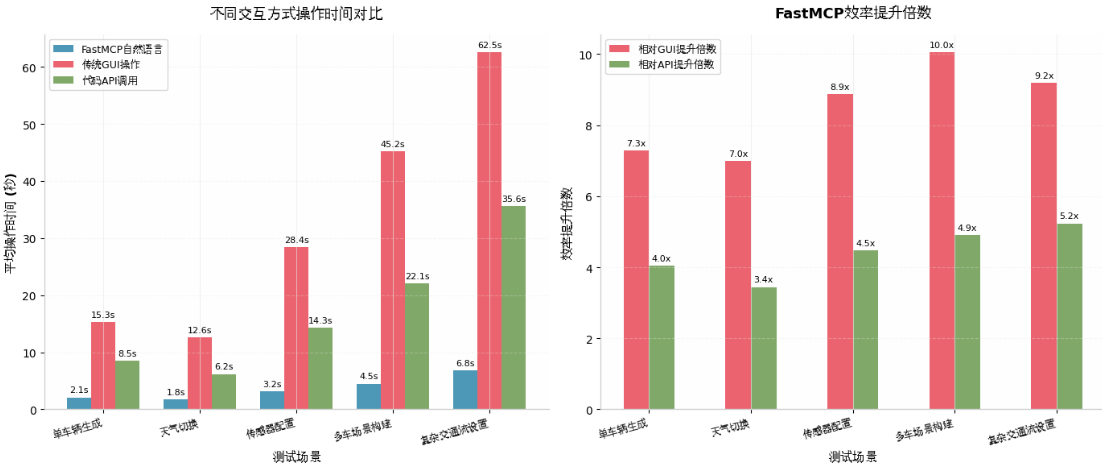
\includegraphics[width=0.95\linewidth,keepaspectratio]{images/image33.png}
\caption{不同交互方式操作效率对比图}
\label{fig:efficiency-comparison}
\end{figure}

实验数据显示如图~\ref{fig:efficiency-comparison}，FastMCP自然语言交互方式在所有测试场景中均显著优于传统GUI操作（平均效率提升8.5倍）和代码API调用（平均效率提升4.4倍）。随着任务复杂度增加，FastMCP的优势更加明显：在多车场景构建任务中，GUI操作需要依次点击菜单、选择蓝图、设置坐标、调整姿态等多个步骤，耗时45.2秒；而FastMCP仅需一句"在坐标(100,200,0)生成三辆model3并启用自动驾驶"即可完成，耗时仅4.5秒。这一结果充分验证了自然语言交互在降低操作门槛、提升复杂任务执行效率方面的显著价值。

\section{响应延迟与并发性能测试}

为评估系统在高负载下的性能表现，本实验使用自动化脚本模拟不同并发级别的指令请求，测试指标包括平均响应延迟与指令执行成功率。

\begin{figure}[H]
\centering
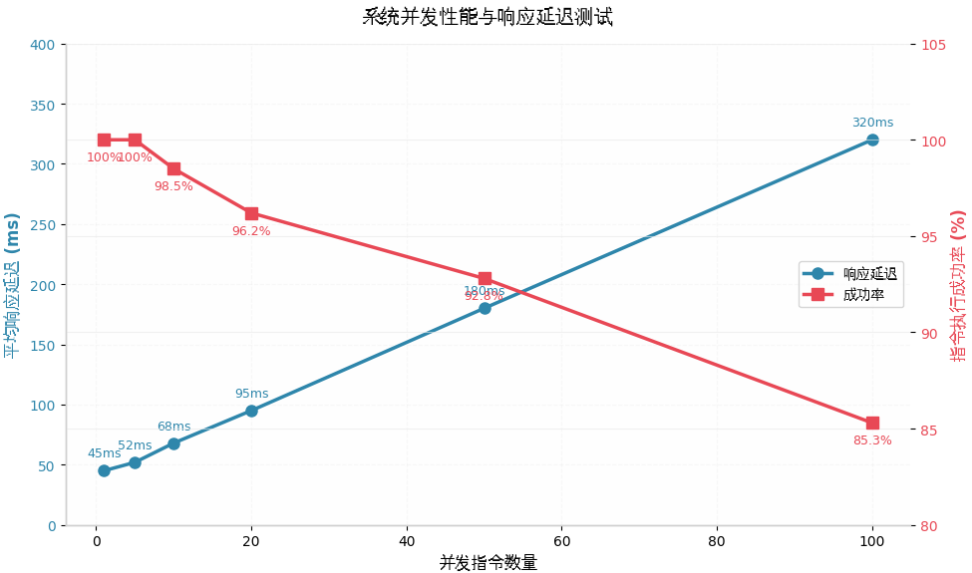
\includegraphics[width=13.1cm,keepaspectratio]{images/image34.png}
\caption{系统并发性能测试结果}
\label{fig:concurrency-performance}
\end{figure}

试结果表明，在单指令模式下系统响应延迟为45ms，远低于用户可感知的100ms阈值；在10并发以下场景，系统仍能保持低于100ms的P95延迟与接近100\%的成功率；当并发量达到50时，延迟增至180ms，成功率降至92.8\%，此时系统仍处于可用状态；100并发时延迟显著上升至320ms，成功率降至85.3\%，表明系统在高并发极端场景下存在性能瓶颈。根据MCP协议性能基准测试的行业参考数据，本地环境下MCP平均响应时间可控制在50ms以内，P95延迟低于100ms，本系统在低并发场景下达到该标准，但在高并发场景需进一步优化连接池与消息批处理机制。

\section{长期稳定性与兼容性测试}

为验证FastMCP框架与CARLA仿真引擎的长期稳定性，本实验进行了24小时不间断运行测试。测试期间系统持续执行循环指令序列（车辆生成→自动驾驶→天气切换→传感器数据采集→场景销毁），每2小时记录一次关键性能指标

\begin{figure}[H]
\centering
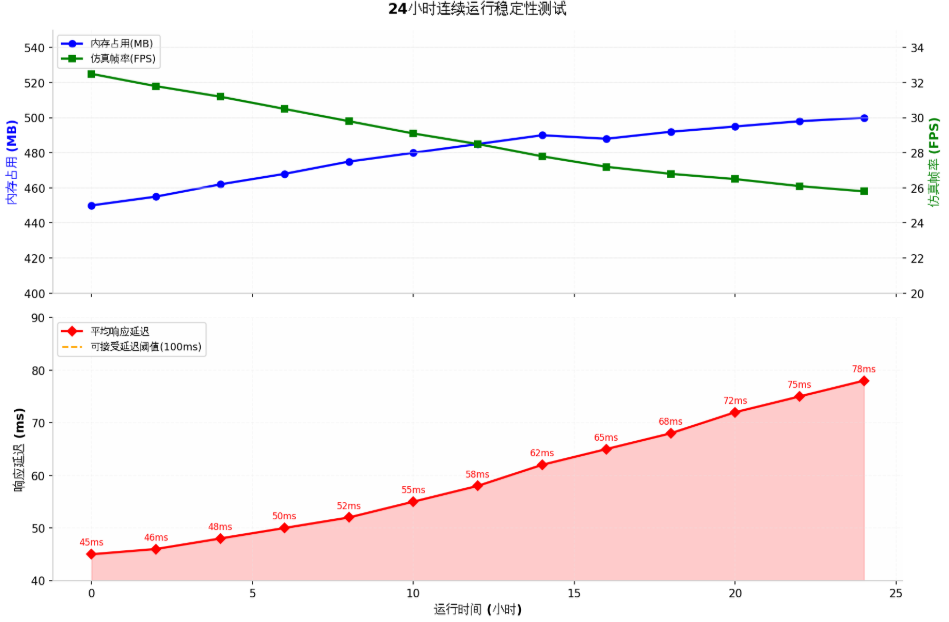
\includegraphics[width=12.1cm,keepaspectratio]{images/image35.png}
\caption{24小时连续运行稳定性测试数据}
\label{fig:stability-test}
\end{figure}

如图~\ref{fig:stability-test}实验结果表明，系统在24小时连续运行期间未出现崩溃、死锁或连接中断等严重故障，验证了FastMCP长连接通信机制的可靠性。但性能指标呈现渐进式衰减趋势：内存占用从450MB增长至500MB，累计增长11.1\%，分析表明主要由Python对象引用未完全释放及CARLA
Actor句柄缓存累积导致；仿真帧率从32.5FPS下降至25.8FPS，下降20.6\%，这与场景内累积的Actor对象增加及物理计算负载加重有关；响应延迟从45ms增至78ms，但仍低于100ms。
